\section{Metodología}
Durante la selección de la metodología a aplicar en este proyecto, se estimó necesario que permitiese la posibilidad de:

\begin{itemize}
    \item \textbf{Anticipación}, en cuanto a la planificación y el producto resultante.
    \item \textbf{Flexibilidad}, en cuanto a la implementación o mejora de funcionalidades.
    \item \textbf{Redacción de una memoria} conforme se desarrolla el proyecto.
\end{itemize}

Teniendo en consideración las características anteriormente mencionadas, se ha escogido la metodología \textbf{iterativa e incremental}. Para comenzar, se toma como referencia el artículo \textbf{\emph{Don't Know What I Want, But I Know Hot to Get It}}~\cite{monalisajp} de Jeff Patton, se analizan los do smétodos que componen dicha metodología.

\begin{itemize}
    \item El \textbf{método incremental} se utiliza con el proposito de encontrar una solución y mejorarla progresivamente. En otras palabras, el desarrollo se efectúa de maneral incremental mediante entregas el usuario utilizará, y a partir de las cuales se recopilará el \emph{\gls{feedback}} para su mejora. Esto permite adaptarse en mayor medida al usuario, partiendo de un punto inicial mas ambigüo y tratando de aproximarnos a la mejor solución posible. Podemos usar como analogía un dibujo, comenzando por el boceto y poco a poco completando la obra tras escuchar las sugerencias del cliente \figref{fig:mona_incremental}.

    \begin{figure}[H]
        \centering
        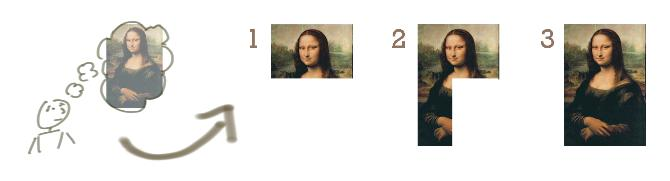
\includegraphics[width=0.8\textwidth]{Ilustraciones/metodologia/patton-incrementing-mona-lisa.jpg}
        \caption{Dibujo incremental de la Mona Lisa por Jeff Patton~\cite{monalisajp}}\label{fig:mona_iterativa}
    \end{figure}

    \item Por otro lado, el \textbf{método iterativo} se utiliza para construir funcionalidades gradualmente. Se desarrolla por entregas, incorporando en cada entrega una nueva funcionalidad. Para ello se debe establecer con bastante rigurosidad los resultados esperados. Si utilizamos nuevamente como referencia el ejemplo del dibujo, se construye poco a poco cada parte de la escena hasta completar la obra \figref{fig:mona_incremental}.
    
    \begin{figure}[H]
        \centering
        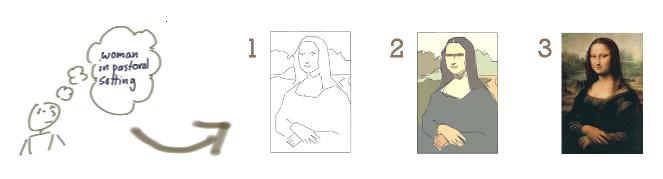
\includegraphics[width=0.8\textwidth]{Ilustraciones/metodologia/patton-iterating-mona-lisa.jpg}
        \caption{Dibujo iterativo de la Mona Lisa por Jeff Patton~\cite{monalisajp}}\label{fig:mona_incremental}
    \end{figure}
\end{itemize}

Si fusionamos los dos métodos obtenemos la \textbf{metodología iterativa e incremental}, la cual nos permite la construcción de software por entregas funcionales donde se implementarán y mejorarán funcionalidades simultáneamente. Continuando con el ejemplo del dibujo, comenzamos por elaborar un boceto y completar poco a poco las partes más importantes, tomando sugerencias del cliente para matizar en los detalles \figref{fig:mona_iterativa_incremental}.

\begin{figure}[H]
    \centering
    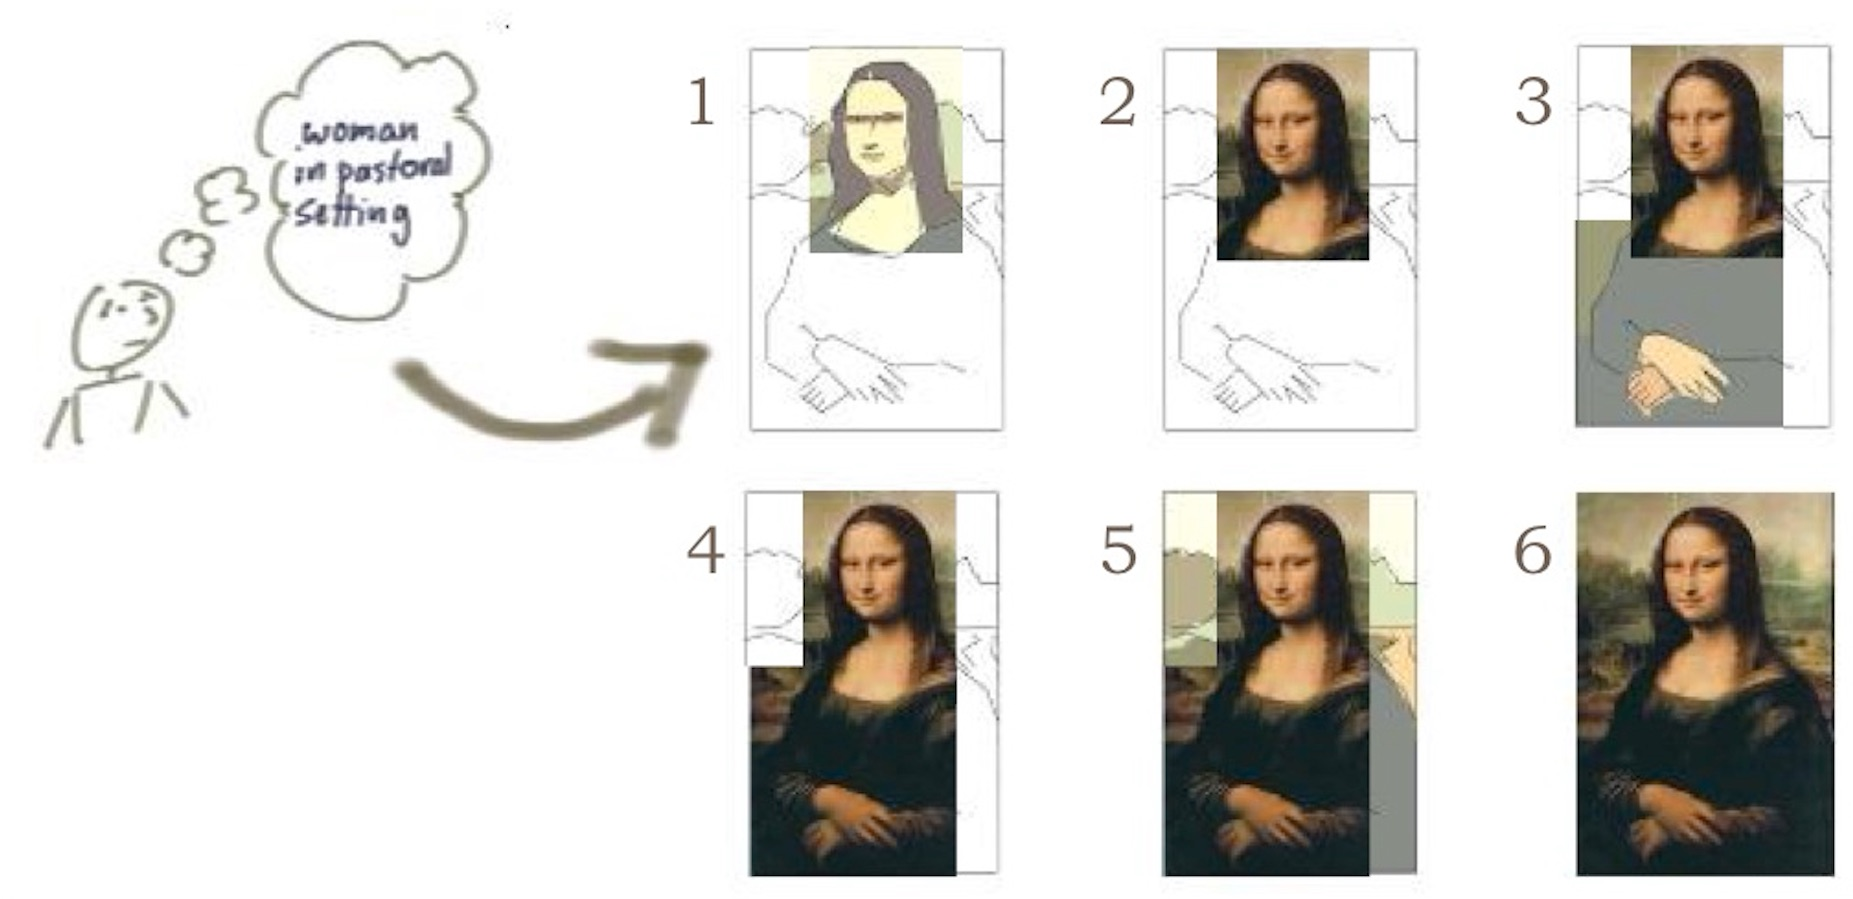
\includegraphics[width=0.8\textwidth]{Ilustraciones/metodologia/iterative-incremental-mona-lisa.jpeg}
    \caption{Dibujo incremental e iterativo de la Mona Lisa por Steven Thomas~\cite{monalisast}}\label{fig:mona_iterativa_incremental}
\end{figure}

Una vez definidos los conceptos que conforman la metodología iterativa e incremental, podemos elaborar el proceso de desarrollo. Este debe incluir las principales \textbf{fases de desarrollo software}; análisis, diseño, desarrollo, pruebas y entrega. Llamaremos \textbf{incremento} a cada repetición del proceso, que implica la implementación o mejora de una funcionalidad. Una vez finalizado el incremento, se entregará al usuario y se decidirá si es necesaria una nueva iteración \figref{fig:flujo_it_inc}.

\begin{figure}[H]
    \centering
    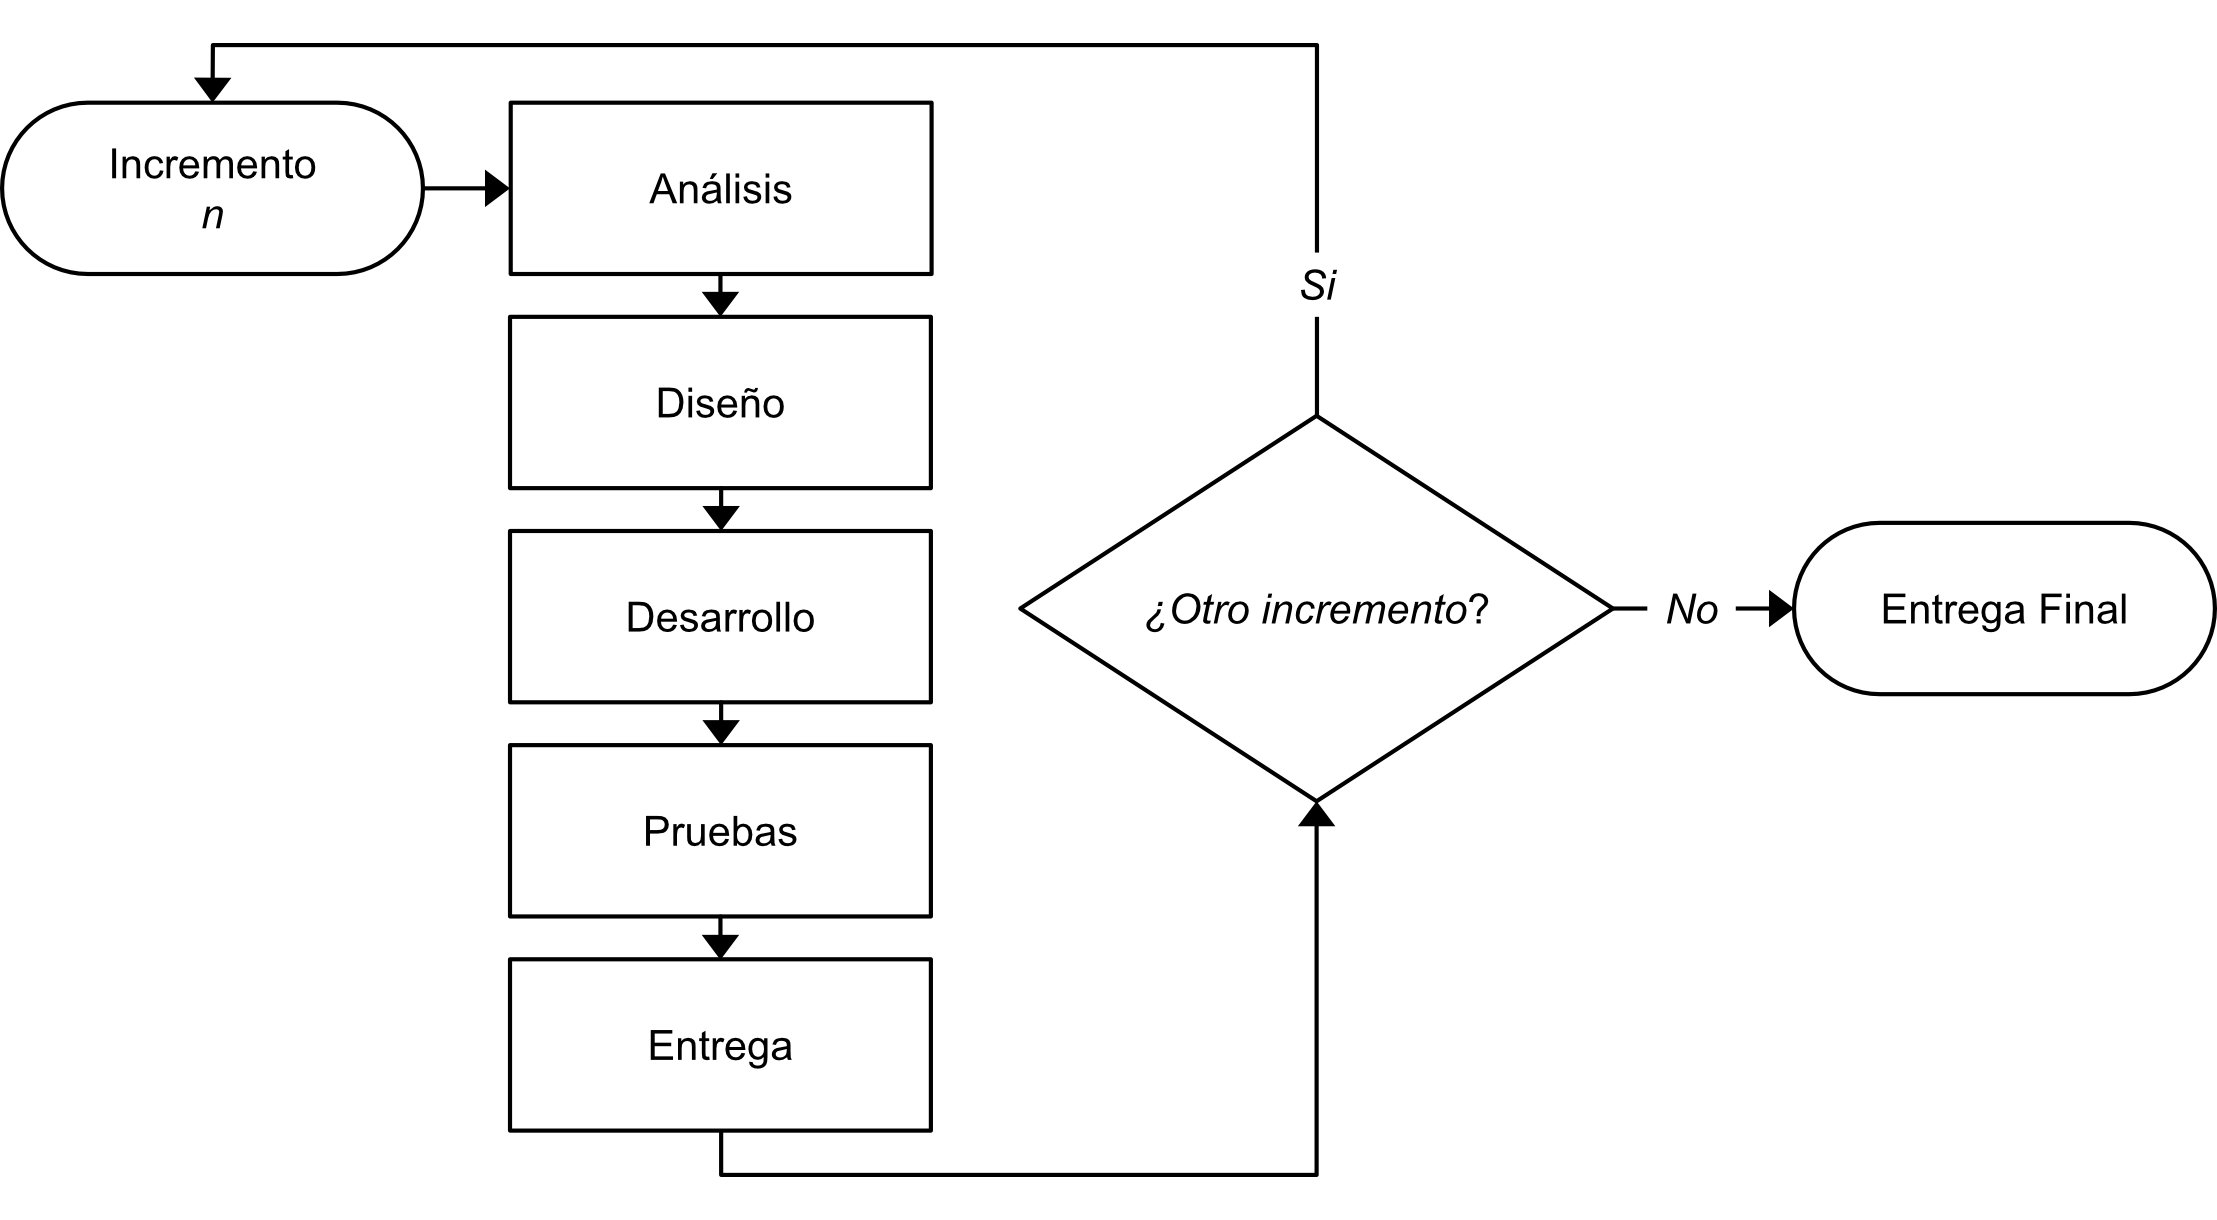
\includegraphics[width=0.8\textwidth]{Ilustraciones/metodologia/flujo_it_inc.jpg}
    \caption{Proceso de desarrollo de la metodología iterativa e incremental}\label{fig:flujo_it_inc}
\end{figure}
